\chapter{Chrétiens et musulmans dans l’Empire ottoman}

\mn{21 mars - Marie Carmen}

\section{Bibiographie}
\begin{itemize}
    \item BOUQUET Olivier,
Pourquoi l’Empire ottoman ? Six siècles d’histoire , Paris,
Gallimard, coll. « Folio », 2022.
   \item
HITZEL Frédéric : 3 livres sur l’histoire ottoman aux éditions Les Belles Lettres.
   \item
L’Empire ottoman. XVe XVIIIe siècles , Paris, Les Belles Lettres,
   \item
Le dernier siècle de l’Empire ottoman (1789 1923), Paris, Les Belles
Lettres, 2014.
   \item
La Turquie au XXe siècle , Paris, Les Belles Lettres,
   \item
GEORGEON
François, V ATIN Nicolas et V EINSTEIN Gilles ( dir .), Dictionnaire
de l’Empire ottoman , Paris, Fayard, 2015. 2 e édition en poche aux éditions du
CNRS, coll. « Biblis », 2022.
\item
LAURENS Henry, TOLAN John et VEINSTEIN Gilles,
L'Europe et
l’islam. Quinze siècles d’histoire. Paris, Odile Jacob, « Hors collection »,
2009 => cf. les chapitres sur l’Empire ottoman rédigés par Gilles Veinstein
\item
Les cours (disponibles en ligne sur le site : au Collègue de France de Gilles
Veinstein (1999 2012) et d’ Edhem Eldem (2017 2022)

\href{https://www.college-de-france.fr/chaire/gilles-veinstein-histoire-turque-et-ottomane-chaire-statutaire}{Gilles
Veinstein Histoire turque et ottomane Collège de France}

\href{https://www.college-de-france.fr/chaire/edhem-eldem-histoire-turque-et-ottomane-chaire-internationale}{Edhem Eldem - Histoire turque et Ottomane}
\end{itemize}


Dans aucun de ces livres, on ne traite la relation entre Chrétiens et musulmans en tant que tels.


\section{Introduction}

\begin{itemize}
    \item Se construit sur les ruines de l'empire Seljoukide
    \item puis en 14 mai 1453, sur les ruines de l'Empire byzantin
\end{itemize}

\paragraph{Soliman le magnifique, Age d'or de l'empire Ottoman au XVI}
\paragraph{Extension maximale au XVII} Une grande partie de la Mediterrannée unifiée.
A noter, Le Maroc n'a jamais été vassal de l'empire Ottoman. 
\begin{figure}[h!]
    \centering
        \sidecaption{L'expansion Ottomane Florian Louis,
Atlas historique
du Moyen Orient , Paris,
Autrement, 2020, p. 46.}
    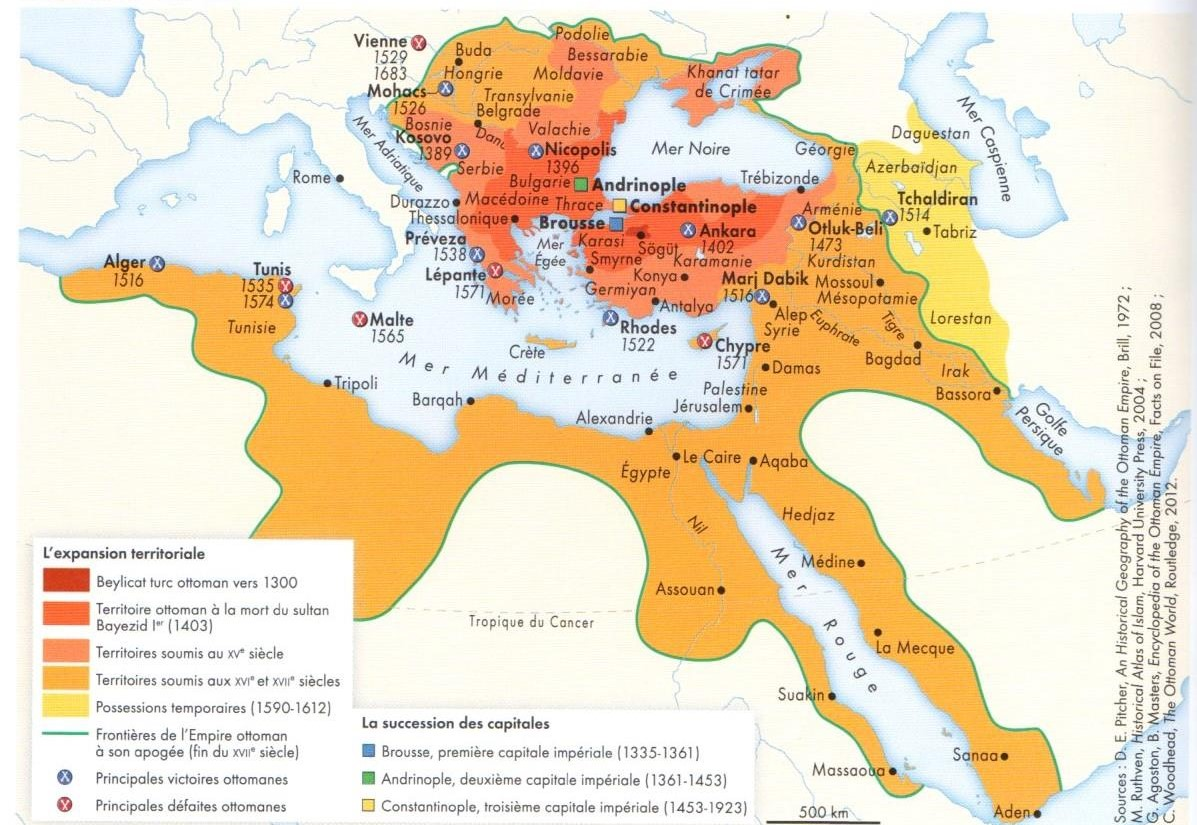
\includegraphics[width=\textwidth]{HistoireIslamMediterranee/Images/ExpansionEmpireOttoman.jpg}

    \label{fig:my_label}
\end{figure}

\begin{figure}[h!]
    \centering
        \sidecaption{L'empire Séfévide et ses voisins au début du XVIIè siècle Florian Louis,
Atlas historique du
Moyen Orient , Paris, Autrement,
2020, p. 47.}
    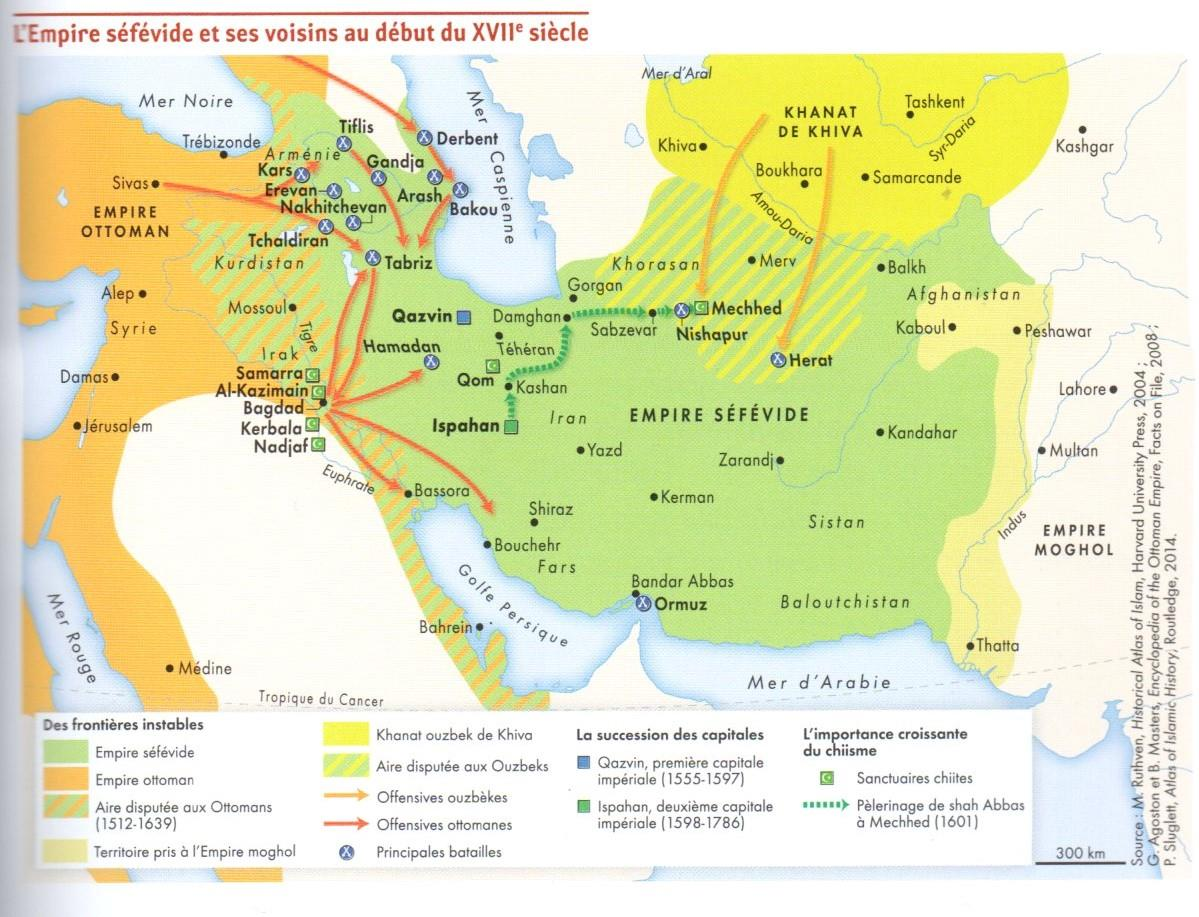
\includegraphics[width=\textwidth]{HistoireIslamMediterranee/Images/EmpireSefevide.jpg}

    \label{fig:my_label}
\end{figure}

\paragraph{Deux grandes batailles} Siège de Vienne au 1683 et Lépante en 1571 (Corinthe). Soliman le pacifique meurt en 1567 et son successeur va avoir à gérer la perte de \href{https://fr.wikipedia.org/wiki/Bataille_de_L%C3%A9pante}{Lépante}.
\begin{figure}[h!]
    \centering
        \sidecaption{L'empire Ottoman au XVIIe}
    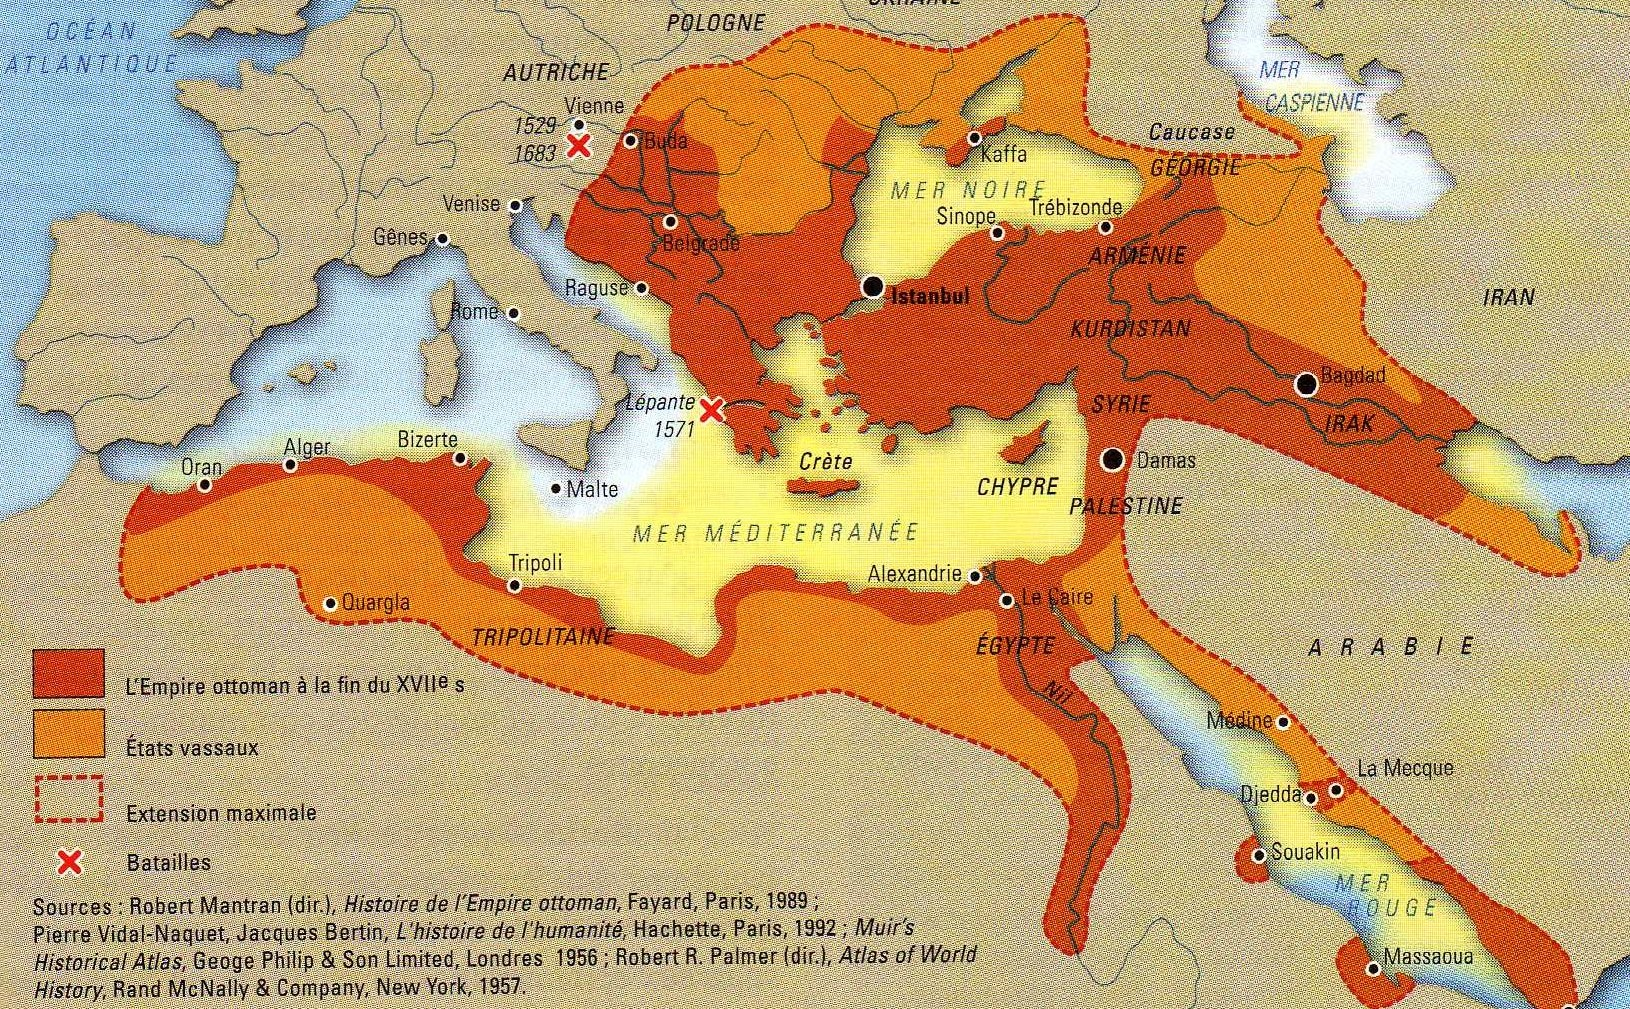
\includegraphics[width=\textwidth]{HistoireIslamMediterranee/Images/EmpireOttomanXVIIe.jpg}

    \label{fig:my_label}
\end{figure}
\paragraph{Peu de sources des début de l'Empire} Tribu d'asie centrale arrivée au moment des Seldjoukides et poussés par les Mongols à entrer dans l'Empire Seldjoukide.
Il y avait des Chrétiens qui parlaient le turc, ce qui a favorisé les premiers liens avec Byzance.



\paragraph{Repère historique}

\begin{itemize}
    \item  
Début des
Tanzimat (réformes) : charte impériale de Gulkhane en
1839 et firman impérial de 1856
    \item  
1876 : Constitution ottomane
    \item  
1889 : Création du Comité Union et Progrès
    \item  
Juillet 1908 : Révolution jeune
turque
    \item  
23 octobre
1923 : Proclamation de la République turque (capitale
Ankara)
\end{itemize}
\section{Encadrer les habitants de l'Empire: communautés et "colonies"}

\paragraph{comment vit on dans un empire pluriel ? } surtout dans le cours au XVIII et XIX : des juifs, des arméniens orthodoxes ou catholiques, ... présence européennes (Vénitiens, Génois, puis français, Anglais,...) et à la fin du XIXè (russe, autrichien, US,...). 

\paragraph{Comment elles s'organisent de façon concrète ? } 
Par le biais de communauté ou de colonies.

\paragraph{Le Millet} pour les communautés éthnico-confessionnelles non musulmanes. 
\begin{itemize}
    \item On met en intermédiaire une structure, et en particulier pour faire remonter les impôts
\end{itemize}

Au départ, 3 millets : 
\begin{itemize}
    \item Grecs
    \item Arménienne Apostolique
    \item juifs
\end{itemize}
\paragraph{Très vite, des problèmes} 3 millets uniquement jusqu'à 1831. Deux nouveaux millets : 
\begin{itemize}
    \item Catholiques 1831
    \item Protestants 1850
\end{itemize}
Ces communautés gèrent les communautés de façon concrète. 
On trouve des millets de façon hétérogènes : dans les villes, on va avoir un millet. 
Un juif n'aura que peu de lien avec l'Empire Ottoman car sa vie va être régie par le millet : Grand Rabbin, ... Ecole, mariage, naissance, décès. 
Avec tout le problème de juridiction pour les catholiques par exemple, d'être enterrés dans un cimetière orthodoxe.
Tribunal du Millet. 

\paragraph{jugement} En cas de problème entre deux chrétiens, juridication du millet. Chrétiens / juifs : compliqué. En cas de musulman, c'est le \textit{qadi}

\paragraph{Capitation} c'est le millet qui le gère. 

\paragraph{A la tête du millet, une élection validée par l'Empire} Système d'élection compliquée. 


\paragraph{Villes cosmopolites : Smyrne, Alexandrie} où tous les millets sont représentées

\subsection{Les colonies}

\paragraph{colonie de Génois et de Vénitiens} 

\paragraph{Système de capitulation ottomane} Le sultan dans sa grandeur, statut particulier : consul, vice consul, agent consulaire... et pareil que le millet. Pour l'aider, le traducteur, le \textit{drogman} attaché à la colonie. 
\begin{marginfigure}
    \centering
    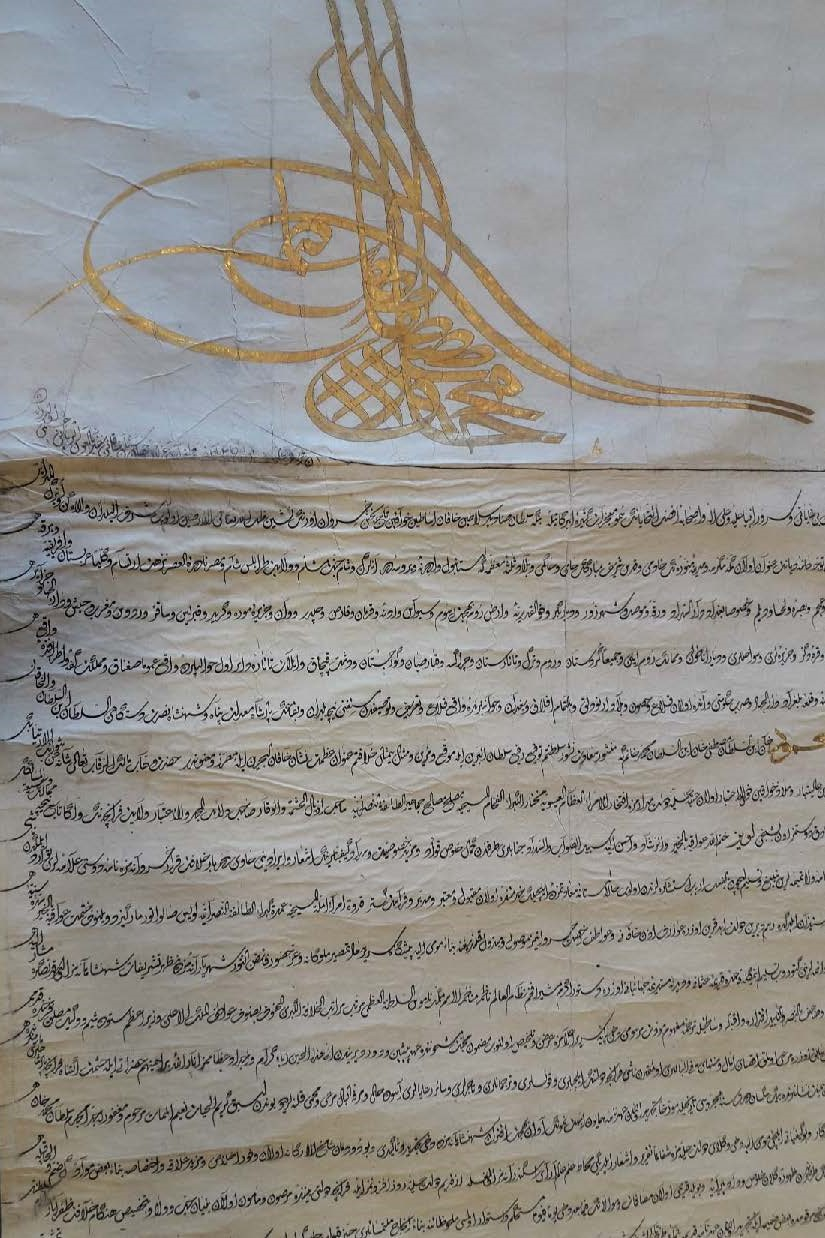
\includegraphics[width=\textwidth]{HistoireIslamMediterranee/Images/firman.jpg}
    \caption{Capitulations ottomanes concédées par le Sultan
Mehmet II au roi Louis XIV le 5 juin 1673
Archives du Ministère français des Affaires
étrangères (La Courneuve)}
    \label{fig:my_label}
\end{marginfigure}
\paragraph{Activités juridiques, notaires} parallèle que le millet. Au XVI, ce sont surtout des hommes, avec l'incitation à ne pas rester ni ne faire des mariages sur place.

\subsection{Réforme}
\paragraph{Privilège} Pour les millets et les colonies, ce sont des privilèges. Rien ne peut être généralisé mais à certaines époques et lieux, des quartiers pour les occidentaux ou les chrétiens, avec des portes fermées.

\paragraph{Début des Tanzimat (réformes)} charte impériale de Gulkhane en 1839 et firman impérial de 1856. 

\paragraph{Question d'orient} Au XIX, intérêt des puissances occidentales à dépecer l'Empire.

\paragraph{Quelles réformes} Par exemple, ouverture de l'armée aux musulmans. Mais possibilité de rachat du service militaire. Mais peu d'occasion pour les non-musulmans pour avoir des interactions avec les musulmans. 

\paragraph{Contrôle au sein du millet} Tous les groupes institutionnels (millet, colonie) interdisent les mariages mixtes pour des raisons religieuses. 
\begin{Ex}
Les Français donnent 10 ans et ne pas avoir le droit de se marier (Marseille).
Cela se faisait à l'\textit{insu du curé} (sic). Ils n'apparaissent pas dans le registre (mais il est sur une feuille volante). 

\end{Ex}
Peu de relations en dehors de la communauté. Au XVII-XVIII, habituel mais au XIXè, cela commence à bouger. 
\paragraph{Des quartiers séparés} comme à Jérusalem, mais partout.

\paragraph{Ce qui nous intéresse, ce n'est pas la règle, c'est la pratique} Pendant très longtemps, on a pensé comme :
\begin{quote}
    {un immeuble où chacun vit chez soi et rencontre son voisin dans le couloir. Malcom Yapp.}
\end{quote}


%-----------------------------------
\section{Coexistences}

\paragraph{Comment fonctionne le vivre ensemble à l'échelle de l'individu} au delà des règles. 
Très peu d'archives dans les villes cosmopolites. On va regarder lazaristes, capucins : analyse très fine : qui se marie avec qui, les témoins, parrains... pour être au plus proche de la réalité.

\paragraph{Dès le XVIII, au delà des interdiction, des liens entre communautés} Des liens existent mais il existe des règles. 

\paragraph{Ce sont souvent les personnes modestes qui transcendent les communautés} des mariages catholiques et orthodoxes dès la fin du XVII au niveau des artisans. Il a aussi des mariages avec des juifs et des ottomans même s'il n'y a pas de trace.
\begin{Ex}
    Une fille juive et un jeune orthodoxe, se marient. horreur ! 
\end{Ex}
Pour les négociants (chic), il faut attendre 1820, avec des mariages catholiques et protestants, et fin du XIX avec les orthodoxes et les grands négociants,...

\paragraph{pareil pour la sociabilité} Trois calendriers, juifs, musulmans, chrétiens, ils ne travaillent que 4 jours ensemble (choc les occidentaux). 
\begin{Ex}
    Les chrétiens viennent dans les quartiers musulmans pour la rupture du jeune. Et inversement, pour Pâques, approprié par tout le monde.
\end{Ex}

\begin{Ex}[club huppé]
    où on se retrouve au XIX avec différentes religions, ce qui est important, c'est d'être chic.
\end{Ex}

\begin{Ex}[Alexandrie]
    Ségrégation ne se fait pas au niveau du quartier (grand négociant,...), la séparation apparaissait au niveau de l'immeuble, le bout de rue. 
\end{Ex}

\paragraph{les conflits ne manquent pas d'éclater} Conflit de voisinage, commerciaux,... On découvre ces conflits dans les registres du qadi, ou du millet, du tribunal consulaire. Cela présuppose qu'il y ait eu des relations.
Si on veut insister sur le fait que cela ne fonctionnait pas, ou si on veut insister sur une perspective pacifique, juste milieu. 

\begin{Ex}[Pâque juive]
    Chaque année, les grecs accusent les juifs de kidnapper les enfants chrétiens et de mélanger leur sang dans le pain azyme. \textit{c'est pas possible, c'est chaque année}
\end{Ex}

\paragraph{Le statut des protégés} Les protégés (barrat) sont des protections individuelles accordées par les consuls. Très prisé et "vendus" ensuite.

\paragraph{1923 : fin des privilèges avec la chute de l'Empire} 



\section{Jeux d'identité}

\mn{Amin Maalouf, entré à l'académie Française, \textit{les identités meurtrières}. }
Pour les voyageurs occidentaux, on ne peut comprendre l'identité plurielle.
Par exemple : un grec orthodoxe : 
\begin{itemize}
    \item Grec orthodoxe : millet orthodoxe
    \item ne parle que le turc mais l'écrive en grec
    \item qui se sont mariés avec une catholique française
    \item dont le père était \textit{protégé} par Naples et lui par la France
    \item reconnu comme Ottoman par l'Empire car vos aïeuls sont arrivés il y a deux siècles. 
\end{itemize}
\paragraph{Quel statut ?}
 Le millet fonctionne sur la religion alors que les capitulations fonctionnent sur la logique nationale. Sans arrêt des problèmes de juridiction.

 \paragraph{Les occidentaux inventent les identités nationales}
 Au milieu du XIXè, des définitions nationales. Une loi pour definir comment on devient ottoman.

 \paragraph{Les pratiques individuelles jouent des identités} Cherchent à sortir des contraintes et les tourner à leur profit. Leur identité est fait de plusieurs identités. 

 \paragraph{Ces identités plurielles sont mises à mal par les lois sur les états nations} Les non musulmans doivent se battre,... A la fin du XIXè, les rapports se dégradent et encore plus avec la révolution \textit{jeunes turcs}. 
 \begin{Ex}[Compétitions sportives]
     opposent différentes communautés. Arméniens contre grecs...
 \end{Ex}

 \paragraph{Massacres commencent au 1897} et le Génocide est en 1916. Rien ne semblait présager cette dégradation. Certes les relations se tendent avec les grecs,...

 \paragraph{les villes cosmopolites disparaissent} Smyrne en 1922. Incendie de la ville chrétienne (ville basse) dans le cadre de la guerre greco-turque. 
 La dernière ville est Beyrouth. 


\paragraph{Le démembrement de
l’Empire ottoman}
\begin{figure}
    \centering
        \sidecaption{Le démembrement de
l’Empire ottoman,
Encyclopédie Larousse}
    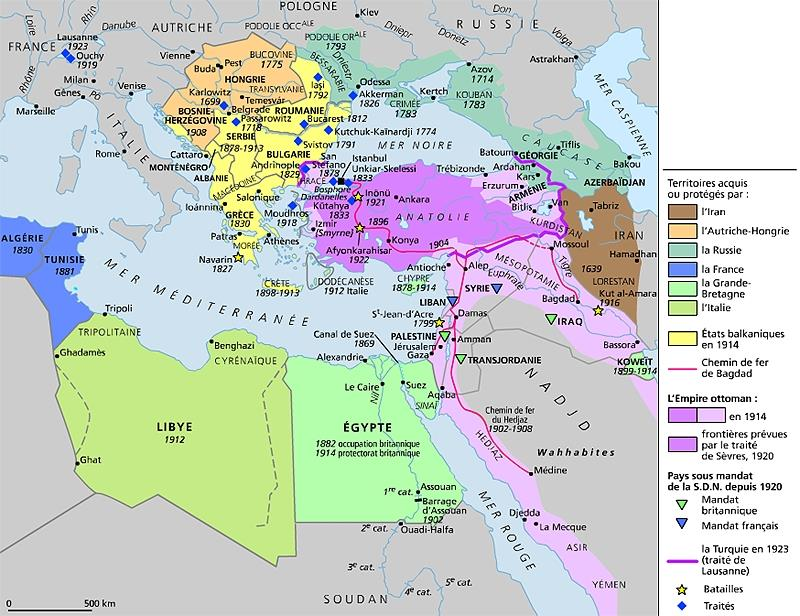
\includegraphics[width=\textwidth]{HistoireIslamMediterranee/Images/DemembrementEmpireOttoman2.jpg}

    \label{fig:my_label}
\end{figure}

 \section{Pour aller plus loin}

 Un documentaire très intéressant d’Arte (2 x 1h) sur l’Empire ottoman
et sa fin (avec des entretiens réalisés avec les meilleurs spécialistes
français et étrangers) :
\href{https://www.dailymotion.com/video/x4a7vu8}{Arte Ottoman 1}
\href{Https://www.dailymotion.com/video/x3zpz4e}{Arte Ottoman 2}

